%!TEX root = main.tex
\setcounter{chapter}{3}
\setcounter{section}{4}
\setcounter{theorem}{0}
\setcounter{equation}{0}

\lectureheader{161}{Calculus I}{Rates of change}{\textit{Thomas' Calculus} \thesection}

\begin{definition}
If $f$ is a function of $x$, then \textbf{instantaneous rate of change of $f$ with respect to $x$ at $x_0$} is
\begin{equation*}
\left.\frac{\dee f}{\dee x}\right|_{x=x_0} = f'(x_0) = \lim_{h\to 0}\frac{f(x_0+h) - f(x_0)}{h}
\end{equation*}
provided the limit exists.
\end{definition}
\begin{remark}
The units of $\frac{\dee f}{\dee x}$ are units of $f$ per units of $x$.
\end{remark}
%\begin{example}
%How fast does the area of a circle change with respect to its diameter when the diameter $D=10$ \si{m}?
%\end{example}
%
%\newpage

\begin{example}
The number of gallons of water in a tank $t$ minutes after the tank has started to drain is
\begin{equation*}
Q(t) = 200(30-t^2).
\end{equation*}
\begin{enumerate}[label=(\alph*)]
\item How fast is the water running out at the end of 10 min?
\vfill
\item What is the average rate at which the water flows out during the first 10 min?
\vfill
\end{enumerate}
\end{example}

\newpage

\begin{example}
Based on data from the U.S. Bureau of Public Roads, a model for the total stopping distance of a moving car in terms of its speed is
\begin{equation*}
s = 1.1v + 0.054 v^2,
\end{equation*}
where $s$ is measured in \si{ft} and $v$ in \si{mph}.
Find and interpret $\left.\frac{\dee s}{\dee v}\right|_{v=35}$ and $\left.\frac{\dee s}{\dee v}\right|_{v=70}$.
\end{example}

\newpage

\begin{definition}
Suppose that an object is moving along a coordinate axis so that its \textbf{position} $s=f(t)$ on that line is a function of time $t$.
\begin{itemize}
\item The \textbf{displacement} of the object over the time interval $[t, t+\Delta t]$ is
\begin{equation*}
\Delta s = f(t+\Delta t) - f(t).
\end{equation*}
\item The \textbf{average velocity} of the object over the time interval $[t, t+\Delta t]$ is
\begin{equation*}
v_{\mathrm{avg}} = \frac{\Delta s}{\Delta t}.
\end{equation*}
\item The \textbf{(instantaneous) velocity} of the object at time $t$ is
\begin{equation*}
v(t) = \frac{\dee s}{\dee t} = f'(t).
\end{equation*}
\item The \textbf{speed} of the object at time $t$ is
\begin{equation*}
|v(t)| = \left|\frac{\dee s}{\dee t}\right| = \left|f'(t)\right|.
\end{equation*}
\item The \textbf{acceleration} of the object at time $t$ is
\begin{equation*}
a(t) = \frac{\dee v}{\dee t} = \frac{\dee^2 s}{\dee t^2} = f''(t).
\end{equation*}
\item The \textbf{jerk} of the object at time $t$ is
\begin{equation*}
j(t) = \frac{\dee a}{\dee t} = \frac{\dee^3 s}{\dee t^2} = f'''(t).
\end{equation*}
\end{itemize}
\end{definition}

\newpage

\begin{remark}
Galileo's experiments suggest that if an object near the Earth's surface is allowed to fall subject only to the Earth's gravity, then the distance fallen after $t$ seconds is
\begin{equation*}
s = \frac{1}{2}g t^2
\end{equation*}
where $g \approx 32$ \si{ft/sec^2} $\approx 9.8$ \si{m/s^2}.
\end{remark}

\begin{example}\,
A ball is released from rest at $t=0$ seconds.
\begin{enumerate}[label=(\alph*)]
\item How far will a ball travel during its first 3 seconds of free fall.
\vfill
\item What is the velocity, speed, and acceleration of the ball at $t=3$ seconds?
\vfill
\vfill
\end{enumerate}
\end{example}

\newpage

\begin{example}
A weight hanging down from a spring is stretched 5 \si{cm} below its rest position and released at time $t=0$.
Its position $t$ seconds later is
\begin{equation*}
s=5\cos t.
\end{equation*}
Compute its velocity, acceleration, and jerk at time $t$.
At what times/positions does its velocity/acceleration/jerk have the greatest magnitude?
\end{example}
\begin{flushright}
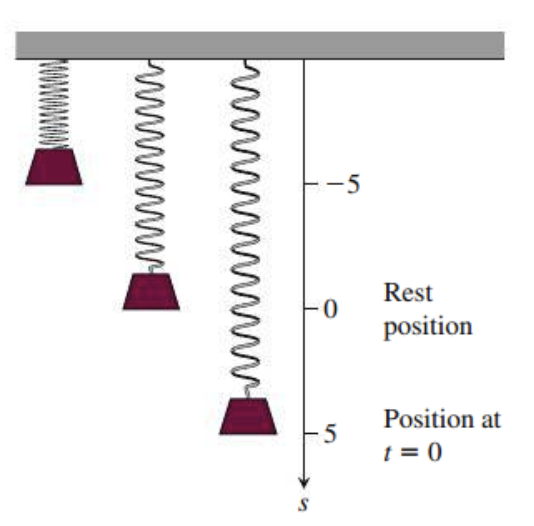
\includegraphics[width=2in]{img/harmonic_motion}
\end{flushright}

\newpage

\begin{example}
The quantity of charge $Q=Q(t)$ in coulombs (C) that has passed through a point in a wire up to time $t$ seconds is
\begin{equation*}
Q = t^3-2t^2+6t+2.
\end{equation*}
Current, measured in amperes (1 \si{A} = 1 \si{C/s}), is the rate of change in current per unit time.
Find the current when $t=1/2$. 
At what time is current the lowest?
\end{example}

\newpage

\begin{remark}
We model a blood vessel as a cylindrical tube with radius $R$ and length $l$.
Due to friction at the walls of the tube, the velocity $v$ of the blood is greatest along the central axis of the tube and decreases as the distance $r$ from the axis increases until $v$ becomes zero at the wall.
Poiseuille's law of laminar flow states that
\begin{equation*}
v = \frac{P}{4\eta l}(R^2-r^2),
\end{equation*}
where $\eta$ is he viscosity of the blood and $P$ is the pressure difference between the ends of the tube.
The \textbf{velocity gradient} is $\frac{\dee v}{\dee r}$, the rate of change in velocity with respect to $r$
\end{remark}

\begin{example}
Compute the velocity gradient assuming that the viscosity, pressure difference, and the tube radius and length are all constant with respect to $r$.
For a small human artery, we might take $\eta=0.027$, $R=0.008$ \si{cm}, $l=2$ \si{cm}, and $P=4000$ \si{dyne/cm^2}.
What is the velocity gradient for this case?
\end{example}

\newpage

\begin{definition}
In a manufacturing operation, the \textbf{level of production} $x$ is the number of units produced and the \textbf{cost of production} $C(x)$ is a function of the level of production.
The \textbf{marginal cost of production} is $\frac{\dee C}{\dee x}$, the rate of change of cost with respect to the level of production.
\end{definition}
\begin{remark}\,
\begin{itemize}
\item The models used in economics are smooth idealizations of discrete ``clumpy" phenomena.
\item The marginals tend not to be extremely sensitive to small perturbations of the input, and so
\begin{equation*}
C'(n)\approx\frac{C(n+1)-C(n)}{(n+1)-n} = C(n+1)-C(n),
\end{equation*}
i.e., the marginal cost when the level of production is $x=n$ is the approximate cost of producing one additional unit.
\item Economists also study marginal demand, marginal revenue, and marginal profit.
\end{itemize}
\end{remark}
\begin{example}
Suppose that a company has estimated that the cost (in dollars) of producing $x$ items is
\begin{equation*}
C(x) = 10000 + 5x + 0.01x^2.
\end{equation*}
Compare the marginal cost at production level $x=500$ items to the actual cost of producing the 501st item.
\end{example}

\newpage

\begin{remark}
\textbf{Predator-prey models} are used to model the interactions between a population of predators and their prey.
\end{remark}
\begin{example}
Consider a population of tundra wolves $W=W(t)$ and caribou $C=C(t)$ at time $t$ in a certain part of northern Canada.
We model their interaction by
\begin{align*}
\frac{\dee C}{\dee t} &= aC-bCW,\\
\frac{\dee W}{\dee t}&=-cW+dCW,
\end{align*}
where $a=0.05$, $b=0.001$, $c=0.05$, and $d=0.0001$.
\begin{enumerate}[label=(\alph*)]
\item What mathematical statement corresponds to both populations being stable?
\vfill
\item How would you represent the statement ``The caribou go extinct" mathematically?
\vfill
\item Find all population pairs $(C,W)$ that lead to stable populations.
According to our model, is it possible for the species to live in harmony or will one or both inevitably become extinct?
\vfill\vfill\vfill\vfill
\end{enumerate}
\end{example}
